%% This is LLNCS.DEM the demonstration file of
% the LaTeX macro package from Springer-Verlag
% for Lecture Notes in Computer Science,
% version 2.4 for LaTeX2e as of 16. April 2010
%
\documentclass{article}

\usepackage[utf8]{inputenc}
\usepackage[top=2.5cm, bottom=2.5cm, left=2cm, right=2cm]{geometry}
\usepackage{graphicx}
\usepackage{color}
\usepackage{float}
\usepackage[small,bf]{caption}
\setlength{\captionmargin}{3pt}
\usepackage{multicol}
\usepackage{blindtext}
\usepackage{geometry}
\usepackage{subfigure}
\usepackage{enumerate}
\usepackage{scalefnt}
\providecommand{\keywords}[1]{\textbf{\textit{Keywords:}} #1}
%
%
\begin{document}

%
%
% ------------------------------------------------------------

\title{An introduction to complex networks with an application study of a co-authorship network obtained from Authenticus}
%
\author{Vanessa Silva\\
	{\texttt{(up201305731@fc.up.pt)}}\\
	\multicolumn{1}{p{.7\textwidth}}{\centering\emph{
		\\Departamento de Ciências de Computadores,\\Faculdade de Ciências da Universidade do Porto}}
}

\date{\today}

\maketitle

% ------------------------------------------------------------

%----------------------ABSTRACT----------------------%

\begin{abstract}
Complex networks is an emergent area of research with high applicability in many areas. In this work, we aim to overview this field of study by introducing the main mathematical concepts, namely of graph theory, that characterize the networks, as well as fundamental properties and laws. Examples of these are: degree, diameter, path, distance, density, connectedness, components, weight, and clustering coefficient, properties such us scale free, power laws, small world, and centrality measures such as betweenness, closeness, and eigenvector.

Within the "world" of complex networks we also made an application study of co-authorship networks, in particular of a network of Portuguese co-authors, obtained from the Authenticus publications database. With the help of Gephi, a graphical tool that has been widely used to view and explore all types of networks and complex systems, it was possible to automatically calculate many of the metrics studied, manipulate and explore the network accordingly to certain metrics and attributes of the network itself, among other possibilities that the software offers.

Finally, we was generated different types of networks in order to study and compare the characteristics of four ISI fields (ISI Web of Science Thomson-Reuters). We concentrated on the areas of Computer Science, Engineering, Mathematics and Physics. We also made a small survey of the evolution of the co-authors networks over a period of 10 years in these areas.

\vspace{3mm}
\keywords{Graphs, complex network, graph theory, nodes, edges, Gephi, Authenticus.}
\vspace{5mm}
\end{abstract}

% ------------------------------------------------------------

\begin{multicols}{2}

%----------------------INTRODUCTION----------------------%

\section{Introduction}

The objective of this work is to study the basics of complex networks, analyze and use some graphical tools that allow the study and comprehension of networks, and make a small study of a network of Portuguese co-authors obtained from the Authenticus.

Complex networks are ubiquitous and subject of research in many scientific areas, namely in computer science, mathematics, physics, biology and sociology. These can be applied to a variety of things that we deal with on a day-to-day, examples of this are the social networks (like the Facebook, LinkedIn and Instagram), biological networks (like the neuronal and metabolic networks) and computer networks (like the Internet).

The study of networks is based on graph theory, first mentioned in 1736 by Leonhard Euler in the paper "Seven Bridges of Königsberg". Over the years there many concepts, strategies and statistical models have been proposed to reason about networks~\cite{NCM, NS}. More recently, techniques and computer resources have facilitated the calculation of metrics, manipulation and visualization of these.

A complex network defines the interactions between the components. Mathematically corresponds to a graph (G) formed by a set of components, called nodes (V), connected by links, called edges (E). The edges can be directed, by connecting two nodes  in which one is the origin and the other is the destination.  Graphs with this feature are called graphs directed or digraphs. The edges may also be undirected, setting only the connection without a direction between the pair of nodes, thus leading to undirected graph or simply graph.  

In a complex system, when we refer to connections we refer to two related issues. A connection may refer to the system structure level, that is, what is connected to what, and a connection may also refer to a behavior level. The fact that the behavior of each system component has implicit consequences on the results of all in the system~\cite{NCM}.

This work presents several graph theory concepts applied to the study of the structure of a complex network, such as paths, cycles, connectivity, components, distance, degree, among other concepts and phenomena.
It also makes a study on the behavior of a complex network. In particular, we do an extensive study of a co-authorship network of Portuguese researchers obtained from the Authenticus platform. Authenticus is a national repository of metadata of scientific publications authored by researchers from Portuguese institutions. It automatically associates authors of publications to researchers and portugueses institutions, but allows researchers to validate these associations, thus assigning the data an increased trust and validity. Currently, its database includes publications of researchers from Portugueses institutions that are indexed in ISI Web-of-Knowledge, Scopus, Crossref and DBLP. The Authenticus also allows two-way synchronization with ORCID of each researcher~\cite{Authenticus}. In our study, we have ensured that at least one co-author belongs to the University of Porto.

A network of co-authorship is a kind of social network that has had considerable interest in many years and has been used to determine the structure of scientific collaborations and to study the status of individual researchers\cite{liu2005co}. Two or more researchers are considered co-authors if there is a common scientific publication between them.

The parsed network is represented by a set of nodes representing the researchers and a set of edges that represent publications done together. When a pair of researchers (nodes) are considered co-authors is created a link (edge) between them.

With the data obtained from Authenticus we generated different types of networks for the different scientific fields, namely Computer Science, Engineering, Mathematics and Physics, aiming to study these networks from a behavioral point of view and also from an evolution point of view. For the later, we generated networks of publications in all areas, one for each year of publications from 2010-2015, in order to be able to accomplish a temporal network study.

All these networks were generated and analyzed with the help of Gephi software, an open-source software that allows analysis and visualization of large networks. It uses a 3D render engine to display graphs in real-time and speed up the exploration. The program offers a set of metrics, real-time preview, filters, layout algorithms and other features for viewing and analysis of complex networks~\cite{Gephi}.

This report is organized as follows. Section~\ref{section.graphtheory} includes a review of the graph theory; section~\ref{section.data} describes the procedures for data manipulation;  section~\ref{section.generation} describes how the networks were generated with Gephi; section~\ref{section.results} presents and  analyses the obtained results; and finally section~\ref{section.conclusions} presents our conclusions and reflections.


%----------------------GRAPH THEORY----------------------%

\section{Graph theory}
\label{section.graphtheory}

Behind each complex system there is a network that encoding the interactions between the system's components. An example of a complex network is the links among Web pages, this can help you understand how these pages are related, how they are grouped into different communities, and which are the most prominent or important.\cite{NS} As well as a network of co-authorship, can be useful to understand how the various investigators are related, how they are grouped into different communities (one example is the scientific areas), and which researchers with greater influence.

For the first example, current Web search engines such as Google, make extensive use of network structure in evaluating the quality and relevance of Web pages. For producing search results, these sites evaluate the relevance of a Web page not only based on the number of links it receives, but based on more subtle aspects of its position in the network. For example, a page can be viewed as more important if receives links from pages that are themselves important.\cite{NS}

The graph theory is a branch of applied mathematics to networks. Studies the relationships among nodes of a graph, which is a mathematical representation of a network.\cite{networklit} The paper "Seven Bridges of Königsberg" by Leonhard Euler, published in 1736, about the problem of the seven bridges of Königsberg, is considered the first result of graph theory.


\subsection{Graph Concepts}

A graph is a set of nodes (or vertices) and a set of edges (or links) that connect pairs of nodes. Using mathematical notation, a graph $G$ can be represented as:
$$G=(V,E)$$
where $V$ is a non-empty set of nodes, and $E$ is a set of edges (a subset of pairs of unordered nodes of $V$).

Two nodes are said to be neighbors, or adjacent, if they are connected by an edge. When there is a direction assigned to the edges, the graph is called directed or digraph. Figure \ref{fig:figure1} illustrates a simple example of a directed graph and figure \ref{fig:figure2} an undirected.

%----------------------FIGURES 1 AND 2----------------------%

\begin{figure*}[ht]
\begin{minipage}[b]{0.5\linewidth}
\centering
\includegraphics[width=5.5cm,height=4cm]{Figures/graph_directed}
\caption{Directed graph (digraph).}
\label{fig:figure1}
\end{minipage}
\hspace{0.5cm}
\begin{minipage}[b]{0.4\linewidth}
\centering
\includegraphics[width=5.5cm,height=4cm]{Figures/graph_undirected_weighted}
\caption{Weighted undirected graph.}
\label{fig:figure2}
\end{minipage}
\end{figure*}

A graph also can be weighted, this means that each edge $(i,j)$ is associated a weight or cost $w_{i,j}$, this weight can be positive or negative. Figure \ref{fig:figure2} illustrates a weighted undirected graph.


\subsection{Degree}

Degree is a very important property of each node of a graph. It represents the number of links (edges) that the node has to other nodes. We denoted by $k_i$ the degree of the $i$th node in the graph~\cite{NS}.

In an undirected graph, the total number of links, $L$, can be expressed as the sum of the node degrees:

$$
L=\frac{1}{2}\sum\limits_{i=1}^{N}k_i
$$

where $N$ is the number of nodes and the factor $\frac{1}{2}$ serves to correct for the fact that in the sum each link is counted twice, for being an undirected and unweighted graph~\cite{NS}.

It should be noted that the description given is for an undirected graph. For digraphs, it is necessary to make the distinction between incoming degree, $k_i^{in}$, and outgoing degree, $k_i^{out}$. The first is the number of edges that point to node $i$, and the second is the number of edges that point from node $i$ to other nodes. The total degree $k_i$ of a node of a digraph is given by~\cite{NS}:

$$
k_i=k_i^{in}+k_i^{out}
$$

In many graphs, one can find some nodes that have a very high degree in relation to other nodes. These nodes are normally called hubs~\cite{networklit}.

We can be also think of calculating the weighted degree of a node. This is a measure that resembles the degree except that here it takes into account the weight of the links, that is, instead of just counting the number of links, it adds up the weights of each connection.


\subsection{Average degree}

The average degree, $\langle k \rangle$, is also a very important property and can be, for undirected graphs, formulated as follows:

$$
\langle k \rangle=\frac{1}{N}\sum\limits_{i=1}^{N}k_i=\frac{2L}{N}
$$


\subsection{Degree distribution}

The degree distribution, $p_k$, gives the probability that a given node has a degree equal to $k$.

$$
p_k=\frac{N_k}{N}
$$

where $N_k$ is the number of nodes with degree $k$, and $N$ is the total number of nodes~\cite{NS}.

A way of presenting degree data is to make a plot of the cumulative distribution function, that is, a frequency counts of occurrence of each degree:

$$
P_k=\sum\limits_{k^{\prime}=k}^{\infty}{p_k}^{\prime}
$$

which represents the probability of a degree being larger or equal to $k$~\cite{newman2003structure}.


\subsection{Path}

A path is a sequence of nodes where each pair of consecutive nodes in sequence is connected by an edge. It can also be helpful to think of a path as a sequence of edges that connect these nodes. Paths can contain nodes repeated or not, without the repeated nodes, paths are called simple path~\cite{NCM}. Each path is constituted by $n+1$ nodes and $n$ edges~\cite{NS}.

A relevant concept is the average path length, $\langle d \rangle$, which is the average of the shortest paths between all pairs of nodes in the graph~\cite{NS}. For a digraph with $N$ nodes, $\langle d \rangle$ is given by

$$
d=\frac{1}{N(N-1)}\sum_{\stackrel{i,j=1,N}{i \neq j}}d_{i,j}
$$

Note that $\langle d \rangle$ is measured only for the node pairs that are in the same component~\cite{NS}.

%----------------------FIGURES 3 AND 4----------------------%

\begin{figure*}[hb]
\begin{minipage}[b]{0.5\linewidth}
\centering
\includegraphics[width=5.5cm,height=4cm]{Figures/graph_disconnected}
\caption{Disconnected graph.}
\label{fig:figure3}
\end{minipage}
\hspace{0.5cm}
\begin{minipage}[b]{0.4\linewidth}
\centering
\includegraphics[width=5.5cm,height=4cm]{Figures/graph_connected}
\caption{Connected graph.}
\label{fig:figure4}
\end{minipage}
\end{figure*}


\subsection{Cycles}

A particular type of non-simple path is a cycle, informally known as the "ring". A cycle is a path with at least three edges, in which the first and last nodes are the same, but all other nodes are distinct~\cite{NCM}.


\subsection{Distance}

The distance between two nodes of a graph is the shortest path length between them, being the path length the number of steps (edges), or the sum of the weights of the edges (if the graph is weighted) that it contains from the origin to the destination, that is, it is a route that runs along the edges of the graph~\cite{NCM, NS}. The shortest path between two nodes $i$ and $j$ is the path with the fewest number of links (edges)~\cite{NS}. Note that there may be more than one.

The calculation of the path must be adapted to the type of graph. In an undirected graph the distance between node $i$ and $j$ is the same as the distance between node $i$ and $j$, $d_{i,j}=d_{j,i}$, while a digraph normally these distances are different, $d_{i,j} \neq d_{j,i}$~\cite{NS}.


\subsection{Diameter}

The diameter, $d_max$, of a graph is defined as the longest shortest path in the graph, that is, the distance between the farthest two nodes~\cite{NS}.


\subsection{Connectivity}

In an undirected graph, nodes $i$ and $j$ are connected if there is a path between them and are disconnected if such a path does not exist. Although there is at least one path between any two nodes on the same cluster, there is no path between nodes belonging to different clusters~\cite{NS}.

A graph is connected if there is a path from each node to all others~\cite{NCM}, and it is disconnected if there is at least one pair of nodes for which is no path that you connect~\cite{NS}.


\subsection{Components}

A connected component is a subset of nodes such that:

\begin{enumerate}[i.]
\item every node in the subset has a path to all others in this subset (component connected internally), and

\item the subset is not part of some larger set with the property that every node can reach all the others~\cite{NCM}.
\end{enumerate}

Suppose a graph contains two distinct components (as shown in figure \ref{fig:figure3}), so, if adding an edge between two nodes, one of each component, it therefore connects the two components, creating a graph with a single component (as shown in figure \ref{fig:figure4}). This link (red edge in the figure) is normally called a bridge. That is, a bridge is any link that, if cut, disconnects the graph~\cite{NS}.


\subsection{Giant Components}

A giant component is a connected component that contains a significant fraction of all nodes of the graph. It is a property often found in large complex networks, and these normally contain only one~\cite{NCM}.


\subsection{Complete graph}

A complete graph is called clique; this type of graph each node is connected to all other nodes. The next figure is illustrated one clique, in particular it is a K5, that is a clique with 5 nodes.

%----------------------FIGURE 5----------------------%

\begin{figure*}
\centering
\includegraphics[width=6cm,height=4.5cm]{Figures/5-clique}
\caption{K5, clique with 5 nodes.}
\label{fig:figure5}
\end{figure*}

In graphs with $N$ nodes, the number of links can vary between $L=0$ and $L_{max}$ in which

$$
L_{max}=\frac{N(N-1)}{2}
$$

In real networks $L$ is much smaller than $L_{max}$, that is, they aren’t represented by cliques~\cite{NS}.


\subsection{Density}

Represents the rate of how many connections exist in the graph in relation to all possible connections. It is a metric that shows how interconnected are the nodes in a graph.

The density of a graph is the relationship between the number of edges, $E$, and the possible number of edges. It is formulated as:

$$
D=\frac{2E}{N(N-1)}
$$

where $N$ is the number of nodes in the graph.


\subsection{Clustering coefficient}

The clustering coefficient is a metric to capture, for a given node, the degree to which the nodes of a graph tend to cluster.

Local clustering coefficient measures how close the neighbors of a given node are to form a clique (complete graph), that is, the degree to which the neighbors of a node interconnect. For a node $i$ with degree $k_i$ local clustering coefficient is given as

$$
C_i=\frac{2L_i}{k_i(k_i-1)}
$$

where $L_i$ is the number of links between the $k_i$ neighbors of node $i$. The value $C_i$ varies between $0$ and $1$, $C_i=0$ if none of the neighbors of node $i$ bind to another node; $C_i=1$ if the neighbors of node $i$ form a complete graph (one click), because they all point to all other nodes; $C_i=0.5$ if there is a $50\%$ probability of two neighboring node $i$ are connected.

With this measure, one can measure the degree of agglomeration (or average network clustering coefficient) of an internal network, since it is captured by the average clustering coefficient $\langle C \rangle$, ($C_i$ averaged over all nodes $i=1,...,N$).

$$
\langle C \rangle=\frac{1}{N}\sum\limits_{i=1}^{N}C_i
$$

Global clustering coefficient measures the total number of closed triangles in the graph. Mathematically it is given by

$$
C_{\Delta}=\frac{3\times number\\of\\triangles}{number \\of \\connected \\triplets}
$$

where triplets represent triplet opened and closed. An open triplet consists of three nodes which are connected by two edges and a closed triplet these nodes are connected by three edges, that is, a triangle.

The factor of $3$ in the formula is due to the fact that each triangle is counted three times in the triplet counting. $C_{\Delta}$ is often called the ratio of transitive triplets~\cite{NS}.


\subsection{Closeness centrality}

The closeness centrality defines how close a node is of all other nodes. To calculate this measure for a given node it is necessary to calculate their shortest path distances to all nodes of the network and reverse these values to a proximity metric (closeness)~\cite{liu2005co}.

%----------------------FIGURES 6 AND 7----------------------%

\begin{figure*}[hb]
\begin{minipage}[b]{0.5\linewidth}
\centering
\includegraphics[width=5.5cm,height=4cm]{Figures/pagerank}
\caption{PageRank.}
\label{fig:figure6}
\end{minipage}
\hspace{0.5cm}
\begin{minipage}[b]{0.4\linewidth}
\centering
\includegraphics[width=5.5cm,height=4cm]{Figures/authorrank}
\caption{AuthorRank.}
\label{fig:figure7}
\end{minipage}
\end{figure*}


\subsection{Betweenness centrality}

This metric determines the number of times a given node is found in the shortest path between any pair of nodes in the graph. Nodes that are often the shortest path between all nodes are considered highly central (control the flow of information in the network)~\cite{liu2005co}.

Betweenness centrality can be seen as a measure of resistance of a graph, which determines how many paths get more minimum when a node is removed from the graph. If nodes are removed, the length of paths between pairs of nodes will increase and thus will be pairs of nodes disconnected. Graphs vary in the level of resistance to such removal. Most are robust to removal of nodes random, but are considerably less robust to removal of nodes with a high degree, core nodes~\cite{newman2003structure}.


\subsection{Eigenvector centrality}

The nodes of a graph aren’t all equal, some are more relevant than others, and therefore have more influence. Eigenvector centrality focuses on the idea that a node is important if it is connected to other important nodes.

A node that has many links do not necessarily have a high value of eigenvector high centrality, because all nodes that are connected to it may have eigenvector centrality low or nil. And a node with high value eigenvector centrality is not necessarily highly connected, it may just have few but important adjacent nodes.


\subsection{Modularity}

Modularity shows how well a graph could be decomposed into modular communities. A high value of modularity indicates a graph with a complete structure of internal communities.


\subsection{AuthorRank and PageRank}

Both AuthorRank and PageRank are metrics centrality.

PageRank is the classification mechanism used by Google~\cite{pagerank98, liu2005co}. It measures the importance of a node by taking into account the quantity and quality of the edges that point to the node. That is, the PageRank value of a node depends on the number of nodes that are connected to it and the PageRank value of these nodes. A node has a high value if there are many nodes that connect to it, and some of these have a high PageRank value. This means that a node is important if there are important nodes connected to it.

$$
PR(A)=\frac{1-d}{N}+d \left(\frac{PR(B)}{L(B)}+\frac{PR(C)}{L(C)}+...\right)
$$

where $N$ is the total number of nodes, $L(x)$ is the number of links of the node $x$, and $d$ is the damping factor.

AuthorRank is a kind of PageRank, but for weighted digraphs. It is based on the hypothesis that a modified node transfers PageRank values uniformly for all nodes to which it is connected. Given this, PageRank assumes that when a node $A$ connects to $N$ nodes, each of which receives a fraction $\frac{1}{N}$ of PageRank $A$, ($PR(A)$). On a weighted network each weight of a link (edge) expresses how strongly related are two nodes in the graph, and these weights are used to determine the PageRank value to be transferred from a node to all its neighbors~\cite{liu2005co, towardsaut2011}.

Figure \ref{fig:figure6} and \ref{fig:figure7} illustrate these two ideas, the first represents the idea of PageRank in which the node transfers the PageRank value uniformly to its neighbors; and the second represents the idea of AuthorRank in which this transfer takes into account the importance of the connection, that is, the weights of the edges.

The AuthorRank of a node $i$ is given by the following mathematical formula:

$$
AR(i)=(1-d)+d\sum\limits_{j=0}^{n}AR(j)\times w_{j,i}
$$

where $AR(j)$ corresponds to AuthorRank node $j$ (adjacent $i$), $w_{j,i}$ represents the weight of the edge connecting these nodes, and $d$ is the damping factor~\cite{liu2005co}.


\subsection{Small-world}

The small world phenomenon resulted from experiments made by Stanley Milgram in the 1960s. The results in which letters passed from person to person were able to reach a target individual in only a small number of steps, around 6 steps were one of the first manifestations of the effect of the small world.

This phenomenon consists of the fact that most of the pairs of nodes, in most networks, appear to be connected by a short path in the network~\cite{newman2003structure}.


\subsection{Scale-free}

Scale-free networks are complex networks whose degree distribution, follows the power law (a functional relationship between two quantities, a change of a quantity results in a proportional change in the other quantity), in that most nodes have few connections in contrast with the existence of few nodes with a high degree, that is, nodes with a high degree tend to connect to nodes with a high degree also.

The earliest published example of a scale-free network is probably Price’s network of citations between scientific papers~\cite{newman2003structure}.


\section{Procedure of data manipulation}
\label{section.data}

For the analysis of a co-authorship network of portuguese researchers we used data provided by Authenticus. The dataset included 84,430 different publications, with 41,832 authors and 1,026,177 connections.

We proceeded to the organization of the data for the analysis which required the writing of a set of small auxiliary programs to:

\begin{itemize}
\item Modify the format of the data provided and separating the fields by semi-colons, thus representing it as a table. This allows the data to be presented in Excel or equivalent, and easily imported into the graphical tool, Gephi.

\item Filter this data in order to:
\begin{itemize}
\item Create the file to the edges (edges.csv) with the following fields:
\begin{itemize}
\item Source: source node identifier;
\item Target: target node identifier;
\item PublicId: publication identifier;
\item YEAR: year of publication;
\item ISIField: academic areas identifier;
\item ISI22Field: category identifier academic areas;
\item Type: network type (directed or undirected), in this case is undirected;
\end{itemize}

\item Create the file to the nodes (nodes.csv) with the following fields:
\begin{itemize}
\item ID: author identifier;
\item RSET: identifier of authors affiliated with the University of Porto (RSET = 1 belongs; RSET = 0 does not belong), provided in the network, at least one researcher in each publication has RSET = 1.
\end{itemize}
\end{itemize}
 
\end{itemize}

After all data are properly organized, in order to generate a complex network, then we proceeded to the generation of the networks. We generated networks for four scientific areas to be analysed in this work. To collect these data, we used small programs.

First, we wrote a program to create files to represent the edges (coauthored links) for each of the networks, this is to filter the above created file (edges.csv) data with PublicId field equal to 5 (Computer Science), 7 (Engineering), 12 (Mathematics) and 18 (Physics). Here, one can also filter by YEAR, for example, to analyze the network at a particular time, and/or another field. We decided to filter the publications between 2000 and 2015 as it was from 2000 that Authenticus began to have more impact, more publications.

Later, we wrote programs to create files representing the nodes belonging to the co-authorship network. These consist of, for the respective file containing the edges of the network one of the areas or the four areas, check the authors (nodes) that are present in this network, verify which of these belong to the University of Porto and finally create the file for each network.

With a similar procedure, we generated networks for each year from 2005 to 2015, that is, ten networks that contain co-authorship links of the year of the publications, in order to verify small temporal changes in the network.

\begin{table*}[ht]
    \begin{minipage}[b]{0.5\linewidth}
        \caption{10 best researchers sorted by degree. 5 represents the of Computer Science area, 7 of Engineering, 12 of Mathematics and 18 the of Physics area. \label{tab:table1}}
        \centering
        
%-----------Table 1------------%
       \begin{tabular}{r|rrrl}

\textbf{ID} & \textbf{RSET} & \textbf{PageRank} & \textbf{\textcolor{red}{Degree}} & \textbf{ISI22Field} \\
\hline

4563 & 0 & 0.00313 & \textcolor{red}{2887} & 7, 18 \\
14273 & 1 & 0.00202 & \textcolor{red}{2186} & 5, 7, 18 \\
16272 &	1 & 0.00317 & \textcolor{red}{2053} & 7, 12, 18 \\
4741 & 1 & 0.00222 & \textcolor{red}{2028} & 5, 7, 18 \\
8668 & 1 & 0.00187 & \textcolor{red}{1958} & 5, 7, 18 \\
15995 & 1 & 0.00212 & \textcolor{red}{1945} & 7, 12, 18 \\
14970 & 1 & 0.00171 & \textcolor{red}{1925} & 5, 7, 18 \\
2280 & 1 & 0.00151 & \textcolor{red}{1876} & 5, 7, 18 \\
14940 & 1 & 0.00141 & \textcolor{red}{1563} & 5, 7, 12, 18 \\
14814 & 1 & 0.00178 & \textcolor{red}{1378} & 7, 18 \\
\hline 
        \end{tabular}
    \end{minipage}
    \hspace{0.5cm}
    \begin{minipage}[b]{0.5\linewidth}
        \caption{10 best researchers sorted by PageRank. 5 represents the of Computer Science area, 7 of Engineering, 12 of Mathematics and 18 the of Physics area. \label{tab:table2}}
        \centering
        
        %-----------Table 2------------%
        \begin{tabular}{r|rrrl}
\textbf{ID} & \textbf{RSET} & \textbf{\textcolor{red}{PageRank}} & \textbf{Degree} & \textbf{ISI22Field} \\
\hline

16272 & 1 & \textcolor{red}{0.00317} & 2053 & 7, 12, 18 \\
4563 & 0 & \textcolor{red}{0.00313} & 2887 & 7, 18 \\
4741 & 1 & \textcolor{red}{0.00222} & 2028 & 5, 7, 18 \\
15995 & 1 & \textcolor{red}{0.00212} & 1945 & 7, 12, 18 \\
14273 & 1 & \textcolor{red}{0.00202} & 2186 & 5, 7, 18 \\
8668 & 1 & \textcolor{red}{0.00187} & 1958 & 5, 7, 18 \\
14814 & 1 & \textcolor{red}{0.00178} & 1378 & 7, 18 \\
14970 & 1 & \textcolor{red}{0.00171} & 1925 & 5, 7, 18 \\
7607 & 1 & \textcolor{red}{0.00158} & 1313 & 7, 18 \\
2280 & 1 & \textcolor{red}{0.00151} & 1876 & 5, 7, 18 \\    
\hline            
        \end{tabular}
    \end{minipage}
\end{table*}


%----------------------GENETATION OF NETWORKS----------------------%

\section{Generation of Networks}
\label{section.generation}

Having all the necessary data, we generated networks in Gephi. Here we exported the files relating to the nodes and edges, and held the following tasks for a better view and analysis of networks:

\begin{itemize}
\item Execute the Fruchterman Reingold layout algorithm in order to separate the different components, with the following values:
\begin{itemize}
\item Area: 20000;
\item Gravity: 1;
\item Speed: 10.
\end{itemize}
\item Execute the Noverlap layout algorithm to try to adjust the overlapping nodes, with the following values:
\begin{itemize}
\item Speed: 3;
\item Ratio: 1.2;
\item Margin: 5.
\end{itemize}
\item Calculate all possible metrics.
\item Put the size and color of the nodes according to their degree, the higher the degree, the greater the size and the darker the color.
\item Repeat the previous parameter for measuring PageRank.
\end{itemize}

With Gephi extract all values and corresponding graphs to the calculated metrics, and tables with the degree and PageRank of each node, for later analysis.


%----------------TABLE 3--------------%

\begin{table*}[hb]
\centering
\caption{Summary of all metrics calculated. CS represents the of Computer Science area, E of Engineering, M of Mathematics, P of Physics and ALL of all areas.}
\label{tab:table3}
\vspace{0.1cm}
\scalefont{0.85}
\begin{tabular}{p{5cm}|p{1.7cm}p{1.7cm}p{1.7cm}p{1.7cm}p{1.7cm}}

\textbf{Metrics} & \textbf{M} & \textbf{CS} & \textbf{P} & \textbf{E} & \textbf{ALL}\\
\hline

\textbf{Average Degree} & 8.011 & 15.013 & 27.645 & 23.544 & 34.541 \\
\textbf{Avg. Weighted Degree} & 8.011 & 15.013 & 27.645 & 23.544 & 34.541 \\
\textbf{Avg. Clustering Coefficient} & 0.761 & 0.731 & 0.746 & 0.713 & 0.705 \\
\textbf{Total Triangles} & 2880 & 14998 & 56197 & 80981 & 121379 \\
\textbf{Connected Components} & 172 & 129 & 122 & 114 & 123 \\
\textbf{Eigenvector Centrality} & 0.020 & 0.056 & 0.054 & 0.132 & 0.132 \\
\textbf{Graph Density} & 0.004 & 0.004 & 0,005 & 0.002 & 0.002 \\
\textbf{Modularity} & 0.935 & 0.862 & 0.818 & 0.825 & 0.812 \\
\textbf{Number of Communities} & 202 & 42 & 37 & 43 & 49 \\
\textbf{Diameter} & 23 & 15 & 18 & 13 & 13 \\
\textbf{Radius} & 1 & 8 & 9 & 7 & 7 \\
\textbf{Average Path Length} & 8.355 & 5.583 & 4.956 & 4.812 & 4.783 \\

\end{tabular}
\end{table*}

%----------------------ANALYSIS AND RESULTS----------------------%

\section{Analysis and Results}
\label{section.results}

\subsection{Co-authored network of four scientific areas}
	
In the present study publications of four scientific fields were considered: Computer Science, Mathematics, Physics, and Engineering, published between 2000 and 2015.

The obtained co-authorship networks are shown in figure \ref{fig:figure8}. In all representations, the researchers are represented by nodes and the relations of co-authored publications by edges undirected and unweighted. The first column is a normal representation that does not protrudes any attribute, the second column protrudes colors and size of the nodes depending on the degree value, so that the most collaborative researcher will have a higher node and darker, and the third column depending on the PageRank value for each node. we can verify that each network has only one giant component, as expected.

Figure~\ref{fig:figure9} shows co-authored networks considering the publications between 2000 and 2015. In the first column, the researchers associated with each area are grouped slightly between themselves forming components. Note that the area of Engineering (represented edges with orange color) is associated enough with each of the other areas, as well as Mathematics (purple edges), though a little less.

In the second and third column the size and color of the nodes represent the degree and PageRank value, respectively. The nodes with higher values are represented with a larger size and a lighter color (almost white). Note that the most connected areas correspond Engineering and Physics. Therefore, it is expected that the majority of nodes with larger size (greater degree and PageRank) belong to these areas, which is confirmed in the tables~\ref{tab:table1} and~\ref{tab:table2}.

\end{multicols}

%----------------FIGURE 8--------------%

\begin{figure}[h]
\centering
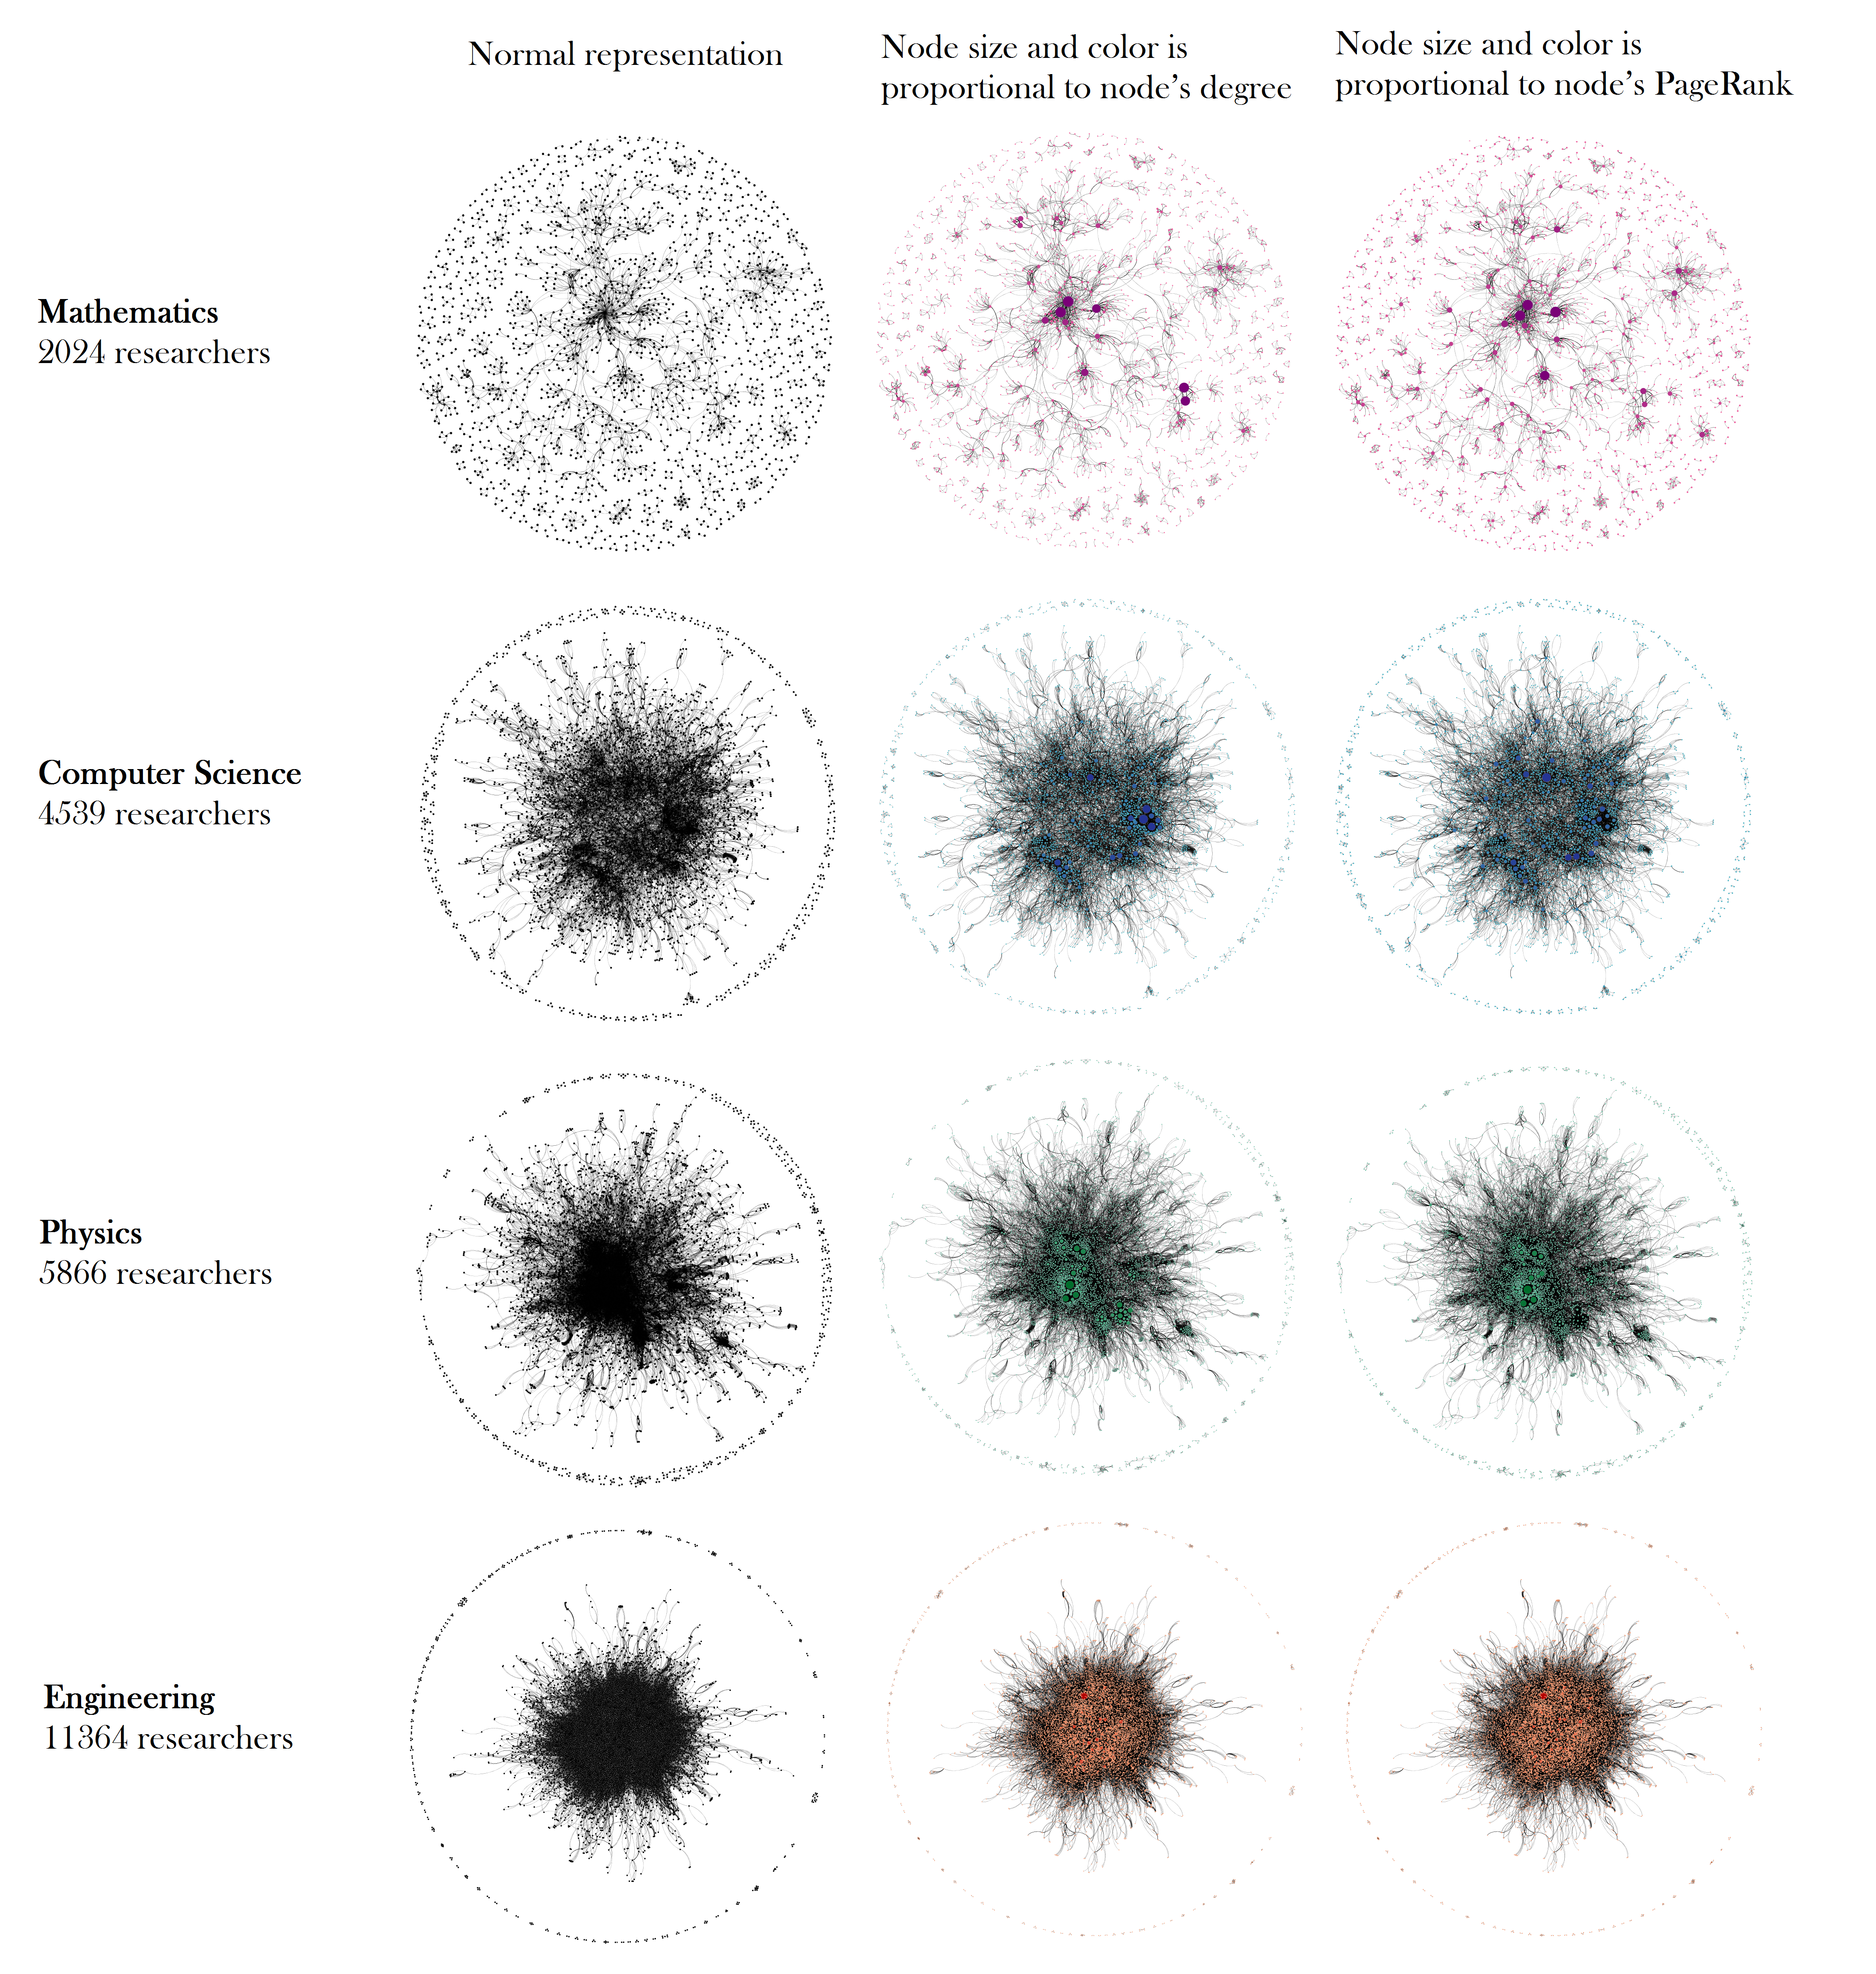
\includegraphics[width=16cm,height=17cm]{Figures/areas}
\caption{Co-authorship networks of Portuguese researchers associated for four scientific fieldss.}
\label{fig:figure8}
\end{figure}


\pagebreak

%----------------FIGURE 9--------------%

\begin{figure}[ht]
\centering
\includegraphics[width=15cm,height=5.5cm]{Figures/ALL}
\caption{Co-authorship networks of Portuguese researchers associated for four scientific fields: Computer Science (blue), Mathematics (purple), Physics(green), Engineering (orange).}
\label{fig:figure9}
\end{figure}


\begin{multicols}{2}

We calculated the Pearson correlation coefficient between the degree and PageRank values, whose value was approximately $0.92$. Note that the metrics show the high connecting an author at the network co-authored.

%% a ultima frase nao se percebe "connecting an author at the network co-authored."

The idea is to verify how strong is the relationship between the two metrics. With the value obtained it can be concluded that there is a strong positive correlation between both variables, which means that if one increases is almost certain that the other increases as well.

We also obtained the value of $R^2= 0.8453$, the coefficient of determination, which says that the variation of degree is represented in approximately $85\%$ by variation of PageRank.

The plot represented in figure \ref{fig:figure10} shows a graphical correlation between the degree and the PageRank of all researchers.

%% inicio de frase estranho, o que se quer dizer?

Compared the representation of co-authorship networks for both measures (degree and PageRank). In the tables \ref{tab:table1} and \ref{tab:table2} are represented the 10 best researchers sorted by PageRank values and degree.

Considering the degree and PageRank value of the nodes, the ten researchers identified are all associated with areas of Physics and Engineering, which was expected, since these are the more connected areas.

Each coauthor network apparently reflects the characteristics of academic practice. For example, the researchers of Mathematics often publish their work with very few co-authors. On the other hand, Physics and Engineering generally tend to have many more co-authors in their publications. One can better understand this idea by calculating the cumulative absolute frequency of the degree of each co-authors network (see plot represented in figure \ref{fig:figure11}). Here it can be seen that the evolution of the curve that represents the area of Physics and the curve representing the Engineering area have very similar and higher values, which reinforces the fact of being the most collaborative areas. The curves that represent the areas of Computer Science and Mathematics are those that have lower values, indicating lower collaboration in these areas, particularly the area of Mathematics.

Only with the degree and PageRank values, we can separate well almost all areas from each other, except for Physics and Engineering that are quite similar. Given this, it is necessary to check if there is another metric that can separate these two areas.

Table \ref{tab:table3}, above, shows all the metrics calculated for each of the networks. It is possible to verify that graph density differentiates well the two areas referred. The density is intended to show how connected are the nodes of a graph. We can say that Physics is more connected (density of $0.005$) than Engineering (with a density of $0.002$).

Note that not all networks form a single connected graph, the majority includes a group (giant component) that occupies more than $90\%$ of all researchers, except for the network that represented the area of Mathematics, where such component takes up only $59.56\%$ of researchers. Given this, the metrics were applied only to the largest connected component, except on the network of Mathematics.


%----------------FIGURE 10 AND 11--------------%

\begin{figure*}[ht]
\begin{minipage}[b]{0.5\linewidth}
\centering
\includegraphics[width=8cm,height=5cm]{Figures/plot1}
\caption{Correlation between the degree and the PageRank.}
\label{fig:figure10}
\end{minipage}
\hspace{0.5cm}
\begin{minipage}[b]{0.5\linewidth}
\centering
\includegraphics[width=8cm,height=5cm]{Figures/plot2}
\caption{Cumulative absolute frequency of the degree of each co-authors network.}
\label{fig:figure11}
\end{minipage}
\end{figure*}


%----------------TABLE 4--------------%

\begin{table*}[hb]
\centering
\caption{Metrics on all networks of publications between 2005 and 2015.}
\label{tab:table4}
\vspace{0.1cm}
\scalefont{0.8}
\begin{tabular}{l|rrrrrrrrrrr}

\textbf{Metrics} & \textbf{2005} & \textbf{2006} & \textbf{2007} & \textbf{2008} & \textbf{2009} & \textbf{2010} & \textbf{2011} & \textbf{2012} & \textbf{2013} & \textbf{2014} & \textbf{2015}\\
\hline

\textbf{Nodes} & 4863 & 6359 & 7443 & 8675 & 9620 & 10130 & 11208 & 12204 & 12770 & 12912 & 12135 \\
\textbf{Edges} & 14033 & 18989 & 23694 & 28211 & 33564 & 40516 & 47162 & 51449 & 49384 & 46477 \\
\textbf{Average Degree} & 6.794 & 6.934 & 7.147 & 7.156 & 7.680 & 7.746 & 7.767 & 8.235 & 8.549 & 8.140 & 8.124 \\
\textbf{Avg. Weighted Degree} & 16.305 & 16.212 & 16.731 & 17.21 & 17.641 & 18.206 & 17.282 & 18.300 & 18.250 & 16.874 & 16.975 \\
\textbf{Average Path Length} & 6.832 & 6.991 & 6.865 & 6.575 & 6.336 & 6.219 & 6.307 & 5.951 & 5.941 & 5.938 & 5.845 \\
\textbf{Network Diameter} & 16 & 20 & 18 & 18 & 18 & 16 & 18 & 17 & 17 & 15 & 19 \\
\textbf{Avg. Clustering Coefficient} & 0.764 & 0.761 & 0.773 & 0.760 & 0.763 & 0.759 & 0.763 & 0.755 & 0.754 & 0.755 & 0.752 \\
\textbf{Modularity} & 0.901 & 0.903 & 0.906 & 0.892 & 0.889 & 0.881 & 0.879 & 0.863 & 0.859 & 0.855 & 0.852 \\
\textbf{Graph Density} & 0.002 & 0.001 & 0.001 & 0.001 & 0.001 & 0.001 & 0.001 & 0.001 & 0.001 & 0.001 & 0.001 \\
\textbf{Connected Components} & 319 & 384 & 35 & 371 & 381 & 410 & 327 & 333 & 301 & 332 & 311 \\

\end{tabular}
\end{table*}


\newpage


\subsection{Co-authored networks between a time period}


Various networks were generated with publications in all ISIField areas, one for each year of publication, from 2005 to 2015, to take place a small time network analysis.

For each of the networks we calculated and compared several metrics (table \ref{tab:table4}). All, except for the metric that provides the number of connected components, for obvious reasons, we calculated for only a component, the giant component. We proceeded like this because in all networks most researchers, more than $75\%$ of these, belong to this component, while the remaining are spread over several smaller components that correspond to one or a few publications, and therefore can be despised in order to have more concise and meaningful results.

From the results obtained (table \ref{tab:table4}) a time comparison may be made, that is, it is possible to analyze how the network evolves over time, comparing the various calculated metrics.

The obtained networks have grown in size almost linearly in just 11 years. There is a small decrease of nodes in the last year, and edges in the last 2 years, probably due to data not being yet all consolidated in Authenticus. Naturally, these networks are expected to increase in terms of researchers and co-authored links between them.

The value of average degree, increases in the first nine years, decreasing slightly in the last two years, which may mean that researchers tend to have more co-authored links over the years. Average weighted degree also tends to increase, although more irregular, there is an almost linear increase from 2006 to 2010 and a sharp decide of the value between 2013 and 2014.

We can also observe that the value of average path length decreases, though slightly, over the years. The values are of the order of $6$ steps observed by Stanley Milgram, showing once again that the co-authored networks possess characteristics of a "Small World". Network diameter varies between $15$ and $20$, being this the size of the longest shortest path in the graph. It remains more or less constant between 2007 and 2013.

The average clustering coefficient values are very close (between $0.75$ and $0.77$), it can show that the co-authorship networks nodes tend to cluster; and modularity values for each network is very close to $1$, which means that the co-authorship networks have a complete structure of internal communities (network divisions).

The number of connected components is between $301$ and $401$, being that the first 6 years have higher values, that is, over the years a co-authorship networks may tend to be connected, having fewer separate components.


\section{Conclusion}
\label{section.conclusions}

In this report we presented a study of complex networks, aiming to consolidate all the concepts involved and to get a better perception of this "world". There are several ways to analyze a complex network, and many network metrics are used in such analysis, namely: degree, path, distance, clustering and centrality. These measures are studied to characterize social networks, identify subcommunities coauthored, or study and characterization of the temporal evolution of the network, among a variety of analysis that can be done.

In order to apply the knowledge acquired, a study was conducted of a co-authorship network of portuguese researchers. First, were analysed four co-authorship networks of publications from four different scientific fields published between 2000 and 2015. We tried to distinguish the different areas using the degree and PageRank metrics. With the help of the Pearson correlation coefficient we verified that both metrics have a strong correlation, and making the cumulative absolute frequency of the degree for each network, we found that all areas can be distinguished, except of the Physics and Engineering that have very close values. For these, we found that the graph density is a metric that can distinguish them, showing that, although both are quite central and connected (alluded properties by PageRank values and degree), the area of Physical is more connected than Engineering area, having Physics a density $0.002$ and Engineering $0.005$.

We also calculated other metrics that may allude to other interesting properties of networks. For example, the scientific communities appear to be a "small world", wherein the average distance between researchers through a series of intermediate researchers, is not more than 5. It is conjectured that this smallness is a fundamental characteristic of a scientific community functional~\cite{newman2001structure}. Another example is the significant value of the average coefficient of grouping (at around $0.7$ for all networks), which shows that two researchers are more likely to be co-authors, if they have a third co-author in common.

In sum, Physics and Engineering are areas with a large collaboration, while the Computer Science and Mathematics tend to have less co-authors in their publications.

Finally, a temporal analysis is made of the network of all publications between 2005 and 2015. 

% Of which can’t make exact conclusions, since were not made statistical predictions, but a small analysis on the set of results obtained from various metrics calculated, for each of the networks.

In this analysis, one can only speculate some changes that a network of co-authorship may have over time. Namely, it is expected to have a value of average path length around 6 so as to be regarded as a network of "Small World". It is also expected that the modularity value is close to 1, since thus it was during 11 years.

Given these temporal data, the analysis of individual publications standards, that is, given a node (researcher) and the number of publications in recent K years, verify whether we can predict how many publications the researcher have the following year, and M years after. This could be a possible study to make.

%The work reported here is one, of many, analysis that can be made with a network co-authors.


% ------------------------------------------------------------

\bibliographystyle{splncs03}
\bibliography{report}
\end{multicols}
\end{document}
